\section{Introduction}
\label{sec:introduction}
Embedded robots combine perception, localization, mapping, planning, and
control on shared compute resources. Heterogeneous platforms provide CPUs,
GPUs, and dedicated neural accelerators, but assigning a workload to an
auxiliary accelerator requires knowing which computation resides there.
A detector intended for the NVIDIA Deep Learning Accelerator (DLA) may still
use GPU kernels.

This work distinguishes nominal DLA deployment from verified fallback-free placement
of the learned graph. TensorRT can request DLA execution while permitting
unsupported regions to fall back to GPU \cite{nvidia_dla_working}. Operator
support, tensor shapes, normalization axes, precision, and I/O layouts constrain
placement. GPU efficiency and successful export do not certify complete
execution on a restricted accelerator.

YOLO11 \cite{jocher2024yolo11} is a representative case: its convolutional
backbone and neck coexist with spatial self-attention and a decoded prediction
interface. Attention matrix products and the flattened prediction path obstruct
strict DLA compilation in the tested configuration. The study examines how
localized architectural and interface changes enable complete learned-graph
placement,
and what accuracy, latency, host-side processing, and energy costs follow.

\begin{figure}[t]
    \centering
    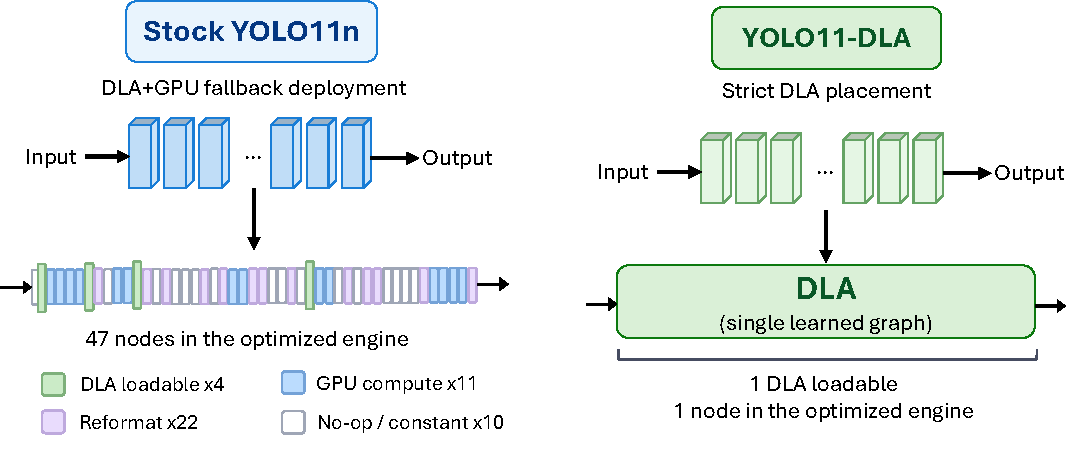
\includegraphics[width=\columnwidth]{figures/teaser.pdf}
    \caption{FP16 deployment. Stock YOLO11n uses DLA+GPU fallback;
    YOLO11-DLA places the complete learned graph in one DLA loadable.
    Host-side decoding and non-maximum suppression remain outside the accelerator.}
    \label{fig:teaser}
\end{figure}

YOLO11-DLA combines architectural adaptation and a static export boundary
for verified placement (Fig.~\ref{fig:teaser}). C2DLA replaces incompatible
spatial attention with channel mixing and local convolution; three raw static
prediction maps define the output boundary. Host-side decoding, confidence
filtering, and non-maximum suppression (NMS) execute on the host. The nano
instance is denoted \model. Recovering GPU capacity for another robotic
workload remains a system-level hypothesis.

This work develops a hardware/software co-design approach for verified
learned-graph placement. First, an architectural adaptation removes accelerator-incompatible
learned computation, and an explicit static prediction boundary separates the
remaining learned graph from host-side decoding and variable-cardinality
post-processing, retaining YOLO11's surrounding architecture and training
formulation. Second, fallback-disabled compilation
and optimized-engine inspection verify placement, while native I/O handling
connects the DLA loadable to the host runtime. Third, deployed-engine evaluation
measures accuracy, engine-plus-transfer latency, application-pipeline latency,
host-side overhead, and module energy at a matched delivered rate in FP16
and calibrated INT8, with GPU controls for both models.
The engine-plus-transfer latency advantage over stock fallback reverses in
application-pipeline latency, demonstrating why placement must be assessed
jointly with accuracy, host-side overhead, and the operating point.
